\section{Round-Robin Testing}

\subsection{Diagramas GANTT}

\begin{enumerate}
	\item lote\_tsk: 5.tsk
	\item num\_cores: 1
	\item switch\_cost: 2
	\item sched\_class: SchedRR
\end{enumerate}

\begin{figure}[h]
    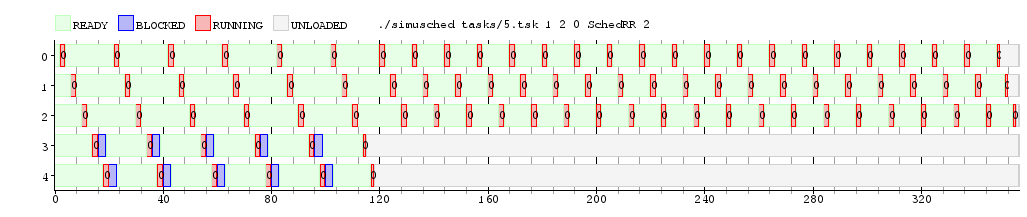
\includegraphics[width=\linewidth]{images/5_quantum2.png}
    \label{fig:Task Consola}
    \caption{Round-Robin (quantum=2)}
\end{figure}

\begin{figure}[h]
    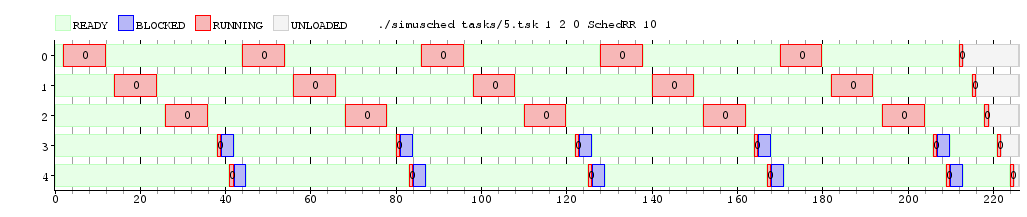
\includegraphics[width=\linewidth]{images/5_quantum10.png}
    \label{fig:Task Consola}
    \caption{Round-Robin (quantum=10)}
\end{figure}

\begin{figure}[h]
    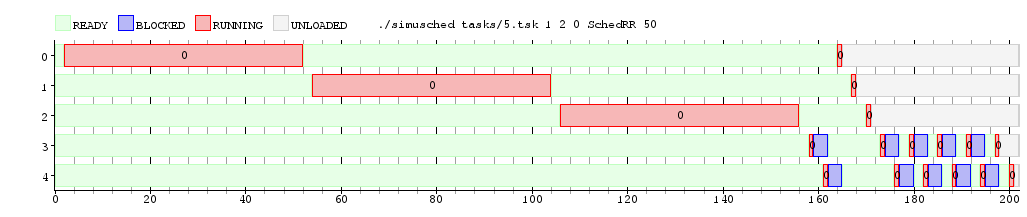
\includegraphics[width=\linewidth]{images/5_quantum50.png}
    \label{fig:Task Consola}
    \caption{Round-Robin (quantum=50)}
\end{figure}

En las 3 figuras anteriores podemos observar los diagramas de Gantt para el algoritmo del scheduler Round-Robin bajo el cual corre un mismo lote (el \textit{lote5}). En los 3 casos se trata de una CPU de un único núcleo, en el cual se tendrá un \textit{switch\_cost} de 2 ciclos de reloj. La particular diferencia entre los 3 es el \textit{quantum} pasado como parametro al Round-Robin; en el que su valor es de 2, 10, 50 respectivamente (según el orden de aparición). Este \textit{quantum} es el que determina cuantos ciclos le son lícitos a cada tarea permanecer en estado \textit{runing}. Ejecutando las tareas de manera alternada por el orden que rige una cola de tareas, cada vez que la CPU se encuentra disponible, se desencola la siguiente tarea y se vuelve a encolar aquella sin finalizar que haya agotado el \textit{quantum} de tiempo asignado. Para un \textit{quantum} no muy grande y tareas que requieran un tiempo no muy corto (menor que el \textit{quantum}), como es el escenario que figura en los 3 diagramas anteriores, el Round-Robin reduce las latencias, ya que al turnar de manera más \textit{justa} el volumen de tareas, la última no debe lidiar con la espera del tiempo completo de ejecución de sus predecesoras, como ocurre con el FCFS. No obstante, se distribuye un costo extra de intercambio de contexto, que repercute en un aumenta del tiempo total de ejecución del lote, de manera acorde a la frecuencia de conmutación dada por el \textit{quantum}. Experimentalmente esto se hace evidente en los graficos anteriores, en donde en el primer caso, de menor \textit{quantum}, el lote abarca un tiempo significativamente mayor que el de los otros dos casos. A su vez el tercer caso, bajo un \textit{quantum = 50}, mejora levemente su performance contra su predecesor, de \textit{quantum = 10}. Sin embargo, no es buena idea tener un \textit{quantum} demasiado grande, pues la rutina tendería a degenerarse hacia el FCFS.